\begin{table}[]
\centering
\begin{tabular}{|c|c|c|c|c|c|c|}
\hline
Case:        & 10     & 12     & 20     & 30     & 40     & 50     \\ \hline
$\frac{A}{h}$ & 0.0989 & 0.1191 & 0.1981 & 0.2958 & 0.3939 & 0.4874 \\ \hline
\end{tabular}
\caption{\textit{Measured amplitude for the incident waves, normalized with water depth.}}
\label{tab:real_ah}
\end{table}


\subsection{Surface profiles of the runup}
\label{surf_pro}
The images captured with the larger FOVs (A and B) reveals how the breaking of the wave effects the surface in the swash zone. The surface profiles were tracked manually due to difficulties regarding air bubbles near the surface. An image from the experiments is given in Figure \ref{fig:overflate_bilde} which illustrates this problem. Figure \ref{fig:runup_10} shows surface profiles for three different times for the non breaking case 10. The surface seems to be repeatable and smooth for all times.
\begin{figure}[]
        \centering
        ~ %add desired spacing between images, e. g. ~, \quad, \qquad, \hfill etc.
          %(or a blank line to force the subfigure onto a new line)
                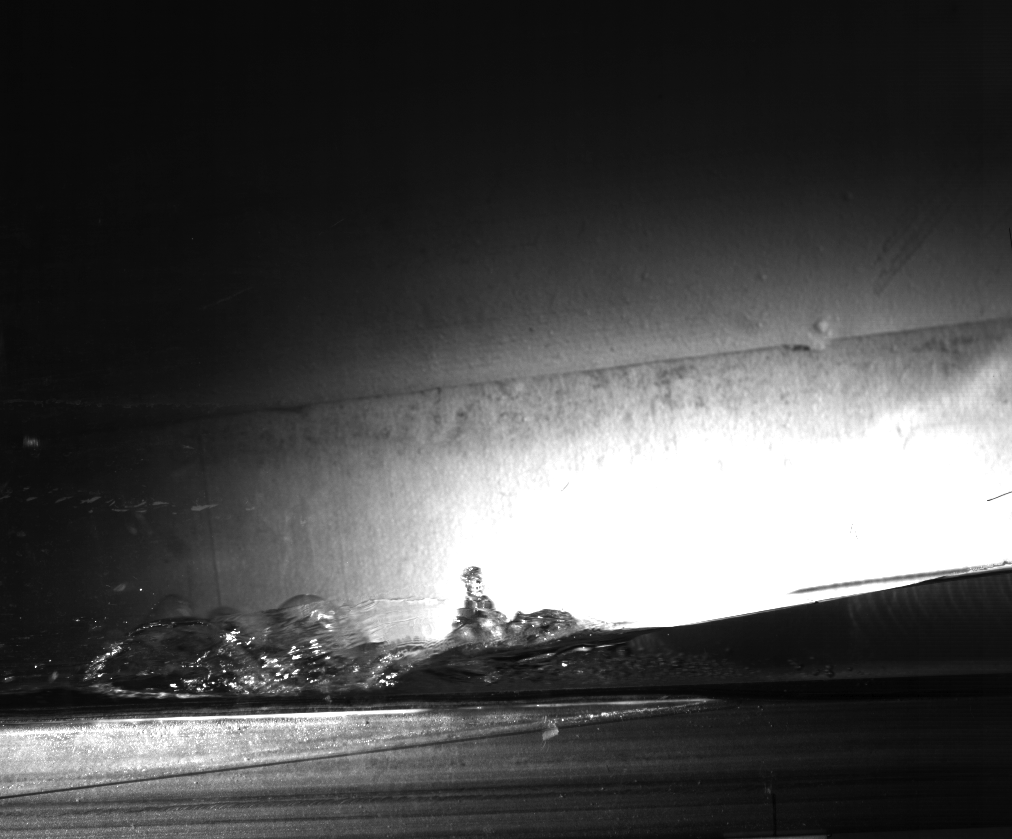
\includegraphics[scale=0.15]{./Figures/overflate_bilde.png}
                \caption{\textit{ Image from FOV A, for case 50 run 1, at t=5.65s }}
                \label{fig:overflate_bilde}
        \end{figure}


\begin{figure}[]
        \centering
         %add desired spacing between images, e. g. ~, \quad, \qquad, \hfill etc.
          %(or a blank line to force the subfigure onto a new line)
        \begin{subfigure}[]{0.4\textwidth}
                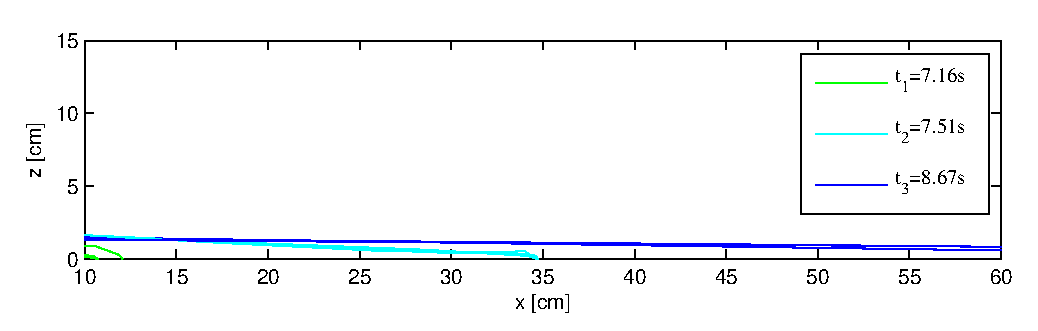
\includegraphics[width=0.9\textwidth]{./Figures/s_p_1A.eps}
                \caption*{\textit{FOV A}}
                \label{fig:overflate_10_1}
        \end{subfigure}
        ~ %add desired spacing between images, e. g. ~, \quad, \qquad, \hfill etc.
          %(or a blank line to force the subfigure onto a new line)
        \begin{subfigure}[]{0.4\textwidth}
                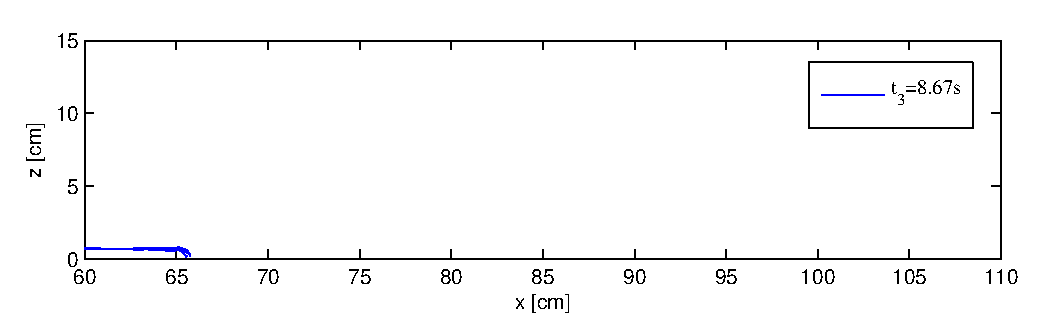
\includegraphics[width=0.9\textwidth]{./Figures/s_p_1B.eps}
               \caption*{\textit{FOV B}}
                \label{fig:overflate_10_2}
        \end{subfigure}
        \caption{\textit{Surface profiles for case 10. Three repetitions are plotted.}}
        \label{fig:runup_10}
\end{figure}
\begin{figure}[]
        \centering
         %add desired spacing between images, e. g. ~, \quad, \qquad, \hfill etc.
          %(or a blank line to force the subfigure onto a new line)
        \begin{subfigure}[]{0.4\textwidth}
                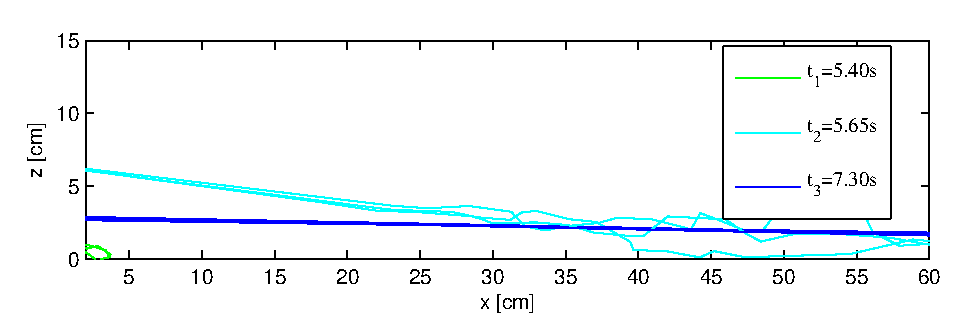
\includegraphics[width=0.9\textwidth]{./Figures/s_p_5A.eps}
                \caption*{\textit{FOV A}}
                \label{fig:overflate_50_1}
        \end{subfigure}
        ~ %add desired spacing between images, e. g. ~, \quad, \qquad, \hfill etc.
          %(or a blank line to force the subfigure onto a new line)
        \begin{subfigure}[]{0.4\textwidth}
                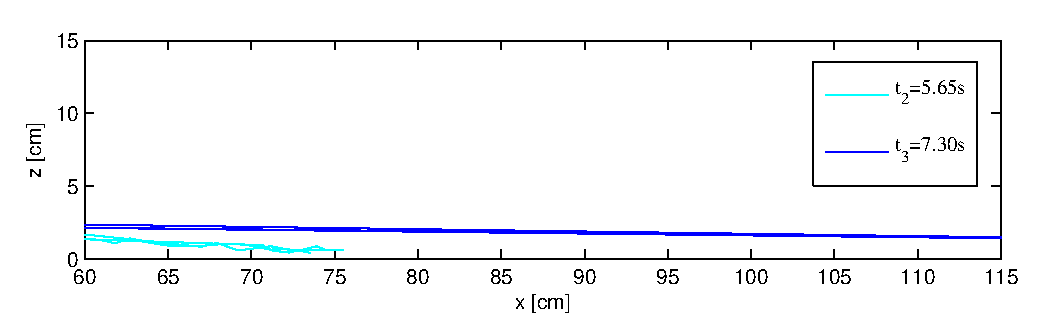
\includegraphics[width=0.9\textwidth]{./Figures/s_p_5B.eps}
               \caption*{\textit{FOV B}}
                \label{fig:overflate_50_2}
        \end{subfigure}
        \caption{\textit{Surface profiles for case 50. Three repetitions are plotted.}}
        \label{fig:runup_50}
\end{figure}
 The surface profiles for the breaking case 50 are shown in Figure \ref{fig:runup_50}. The surface was easy to track and seems to be repeatable for $t_1$. However at $t_2$, the surface was unstable and not repeatable. I believe this is due to inaccuracy in the tracking process of the surface profiles. It was extremely hard to define the surface line when air bubbles were bursting. The surface became steady again when all the air was separated from the water. This made it easier to track the surface again at $t_3$. 